\section{Results}



\subsection{Equilibrium}

\begin{figure}[H]
  \centering
  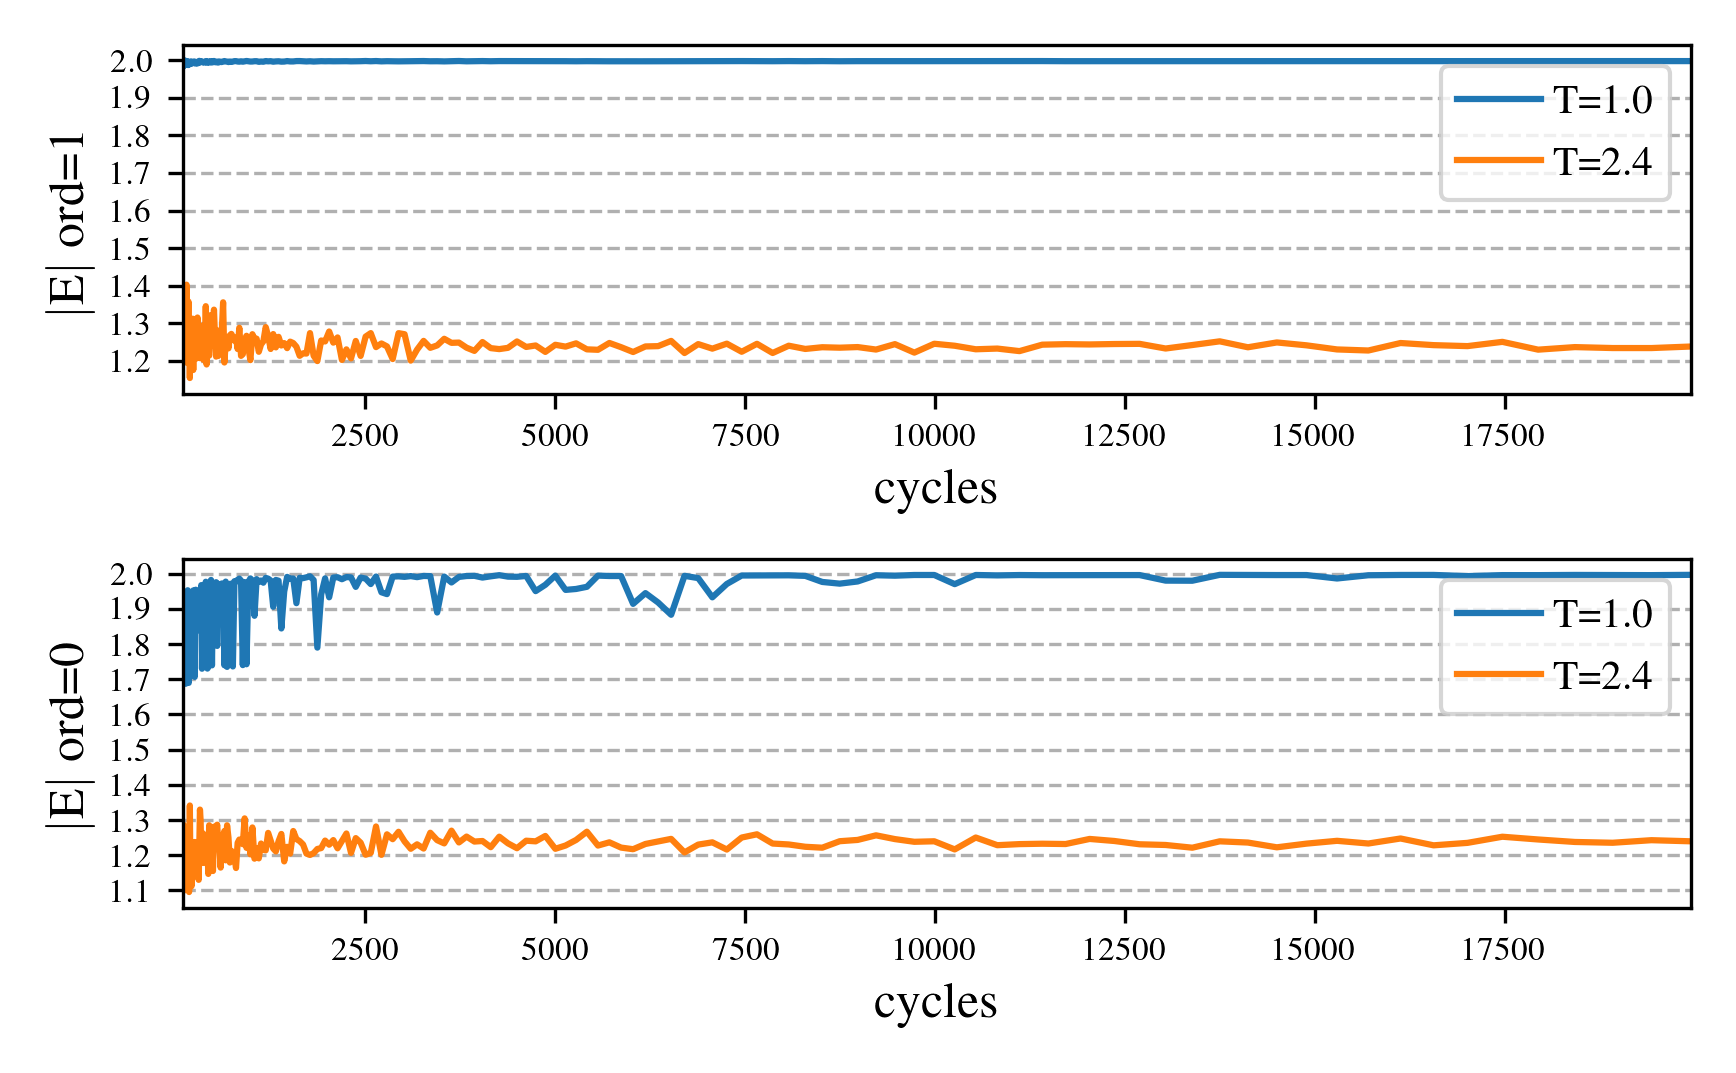
\includegraphics[width=\textwidth]{../figures/equilibrium_E.png}
  \caption{Absolute values of energy for different MC cycles.
  ord refers to the initial configuration of spins. 1=up, -1=down, 0=random.}
  \label{fig:equi_E}
\end{figure}


\begin{figure}[H]
  \centering
  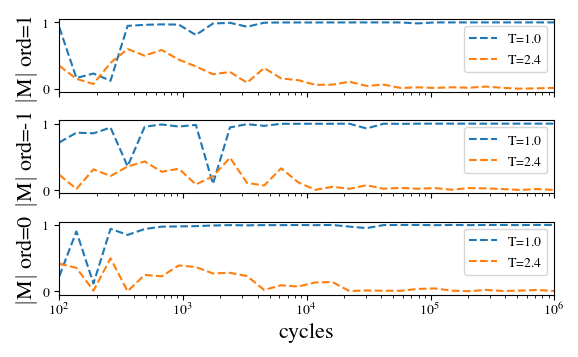
\includegraphics[width=\textwidth]{../figures/equilibrium_M.png}
  \caption{Absolute values of magnetization for different MC cycles.
  ord refers to the initial configuration of spins. 1=up, -1=down, 0=random.}
  \label{fig:equi_M}
\end{figure}


\begin{figure}[H]
  \centering
  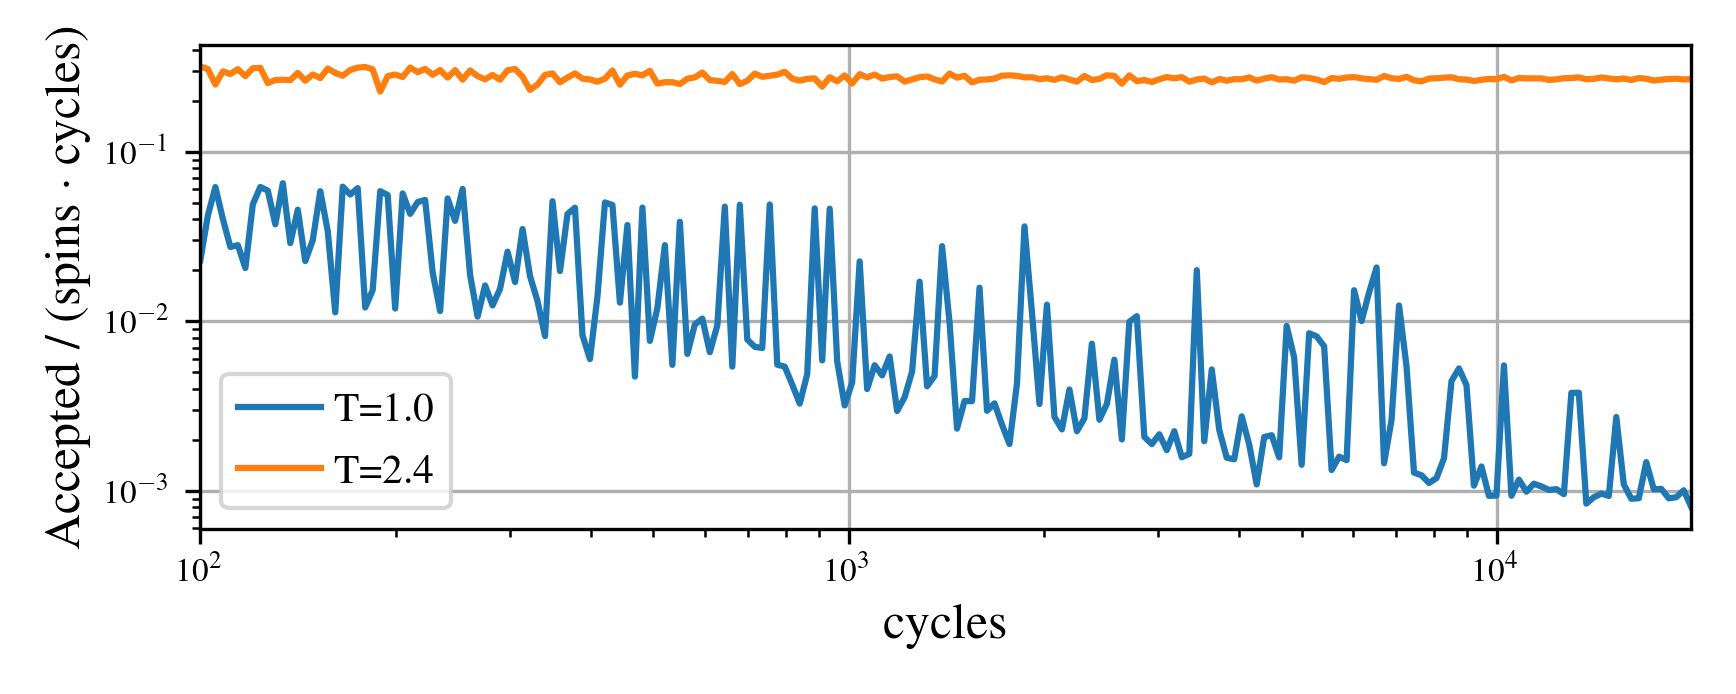
\includegraphics[width=\textwidth]{../figures/accepted.png}
  \caption{Accepted configurations scaled with number of spins and MC cycles.}
  \label{fig:accepted}
\end{figure}


\subsection{Probability distribution}



\begin{figure}[H]
  \centering
  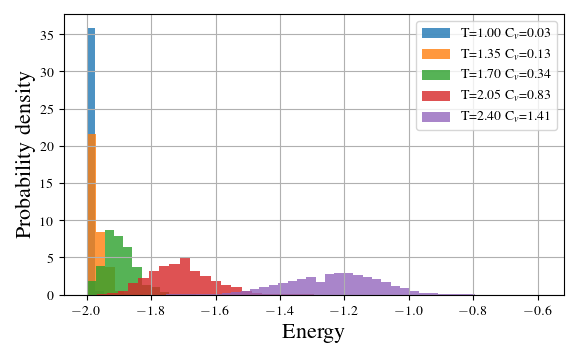
\includegraphics[width=\textwidth]{../figures/distribution.png}
  \caption{Probability distribution of energy, scaled with number of spins.}
  \label{fig:distribution}
\end{figure}




\subsection{Phase transitions}




\begin{figure}[H]
  \centering
  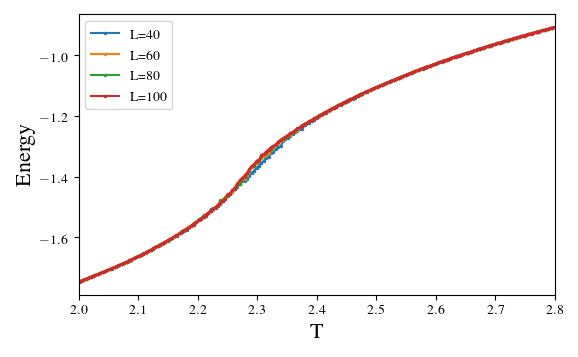
\includegraphics[width=\textwidth]{../figures/phase_E.png}
  \caption{}
  \label{fig:phase_E}
\end{figure}

\begin{figure}[H]
  \centering
  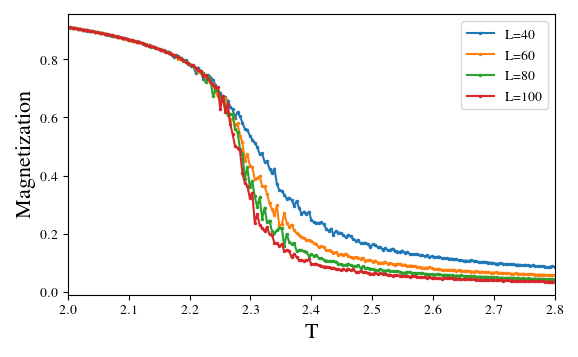
\includegraphics[width=\textwidth]{../figures/phase_Mabs.png}
  \caption{}
  \label{fig:phase_Mabs}
\end{figure}



\begin{figure}[H]
  \centering
  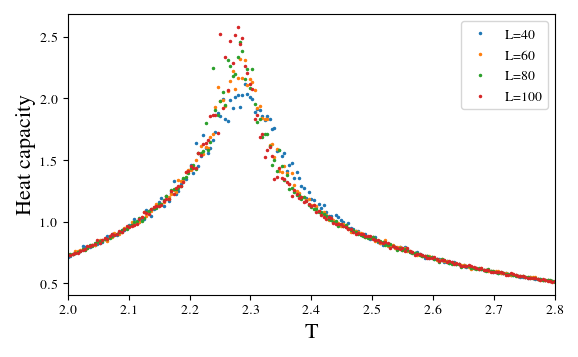
\includegraphics[width=\textwidth]{../figures/phase_cv.png}
  \caption{}
  \label{fig:phase_cv}
\end{figure}


\begin{figure}[H]
  \centering
  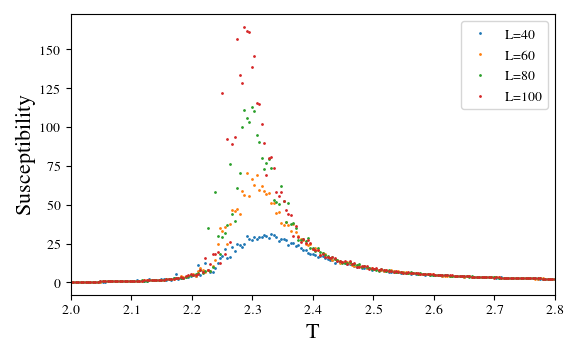
\includegraphics[width=\textwidth]{../figures/phase_suscept.png}
  \caption{}
  \label{fig:phase_suscept}
\end{figure}
